\documentclass[12pt,times,letter]{article}

\usepackage{float}
\usepackage{placeins}
\usepackage{amsmath}
\usepackage{color}
\usepackage{amssymb}
\usepackage{mathtools}
\usepackage{subfigure}
\usepackage{epsfig}
\usepackage{listings}
\usepackage{enumitem}
\usepackage{graphicx}    
\usepackage{graphics}
\usepackage{epstopdf}
\usepackage{longtable}
\usepackage[pdftex]{hyperref}
\usepackage{breakurl}
\usepackage{epigraph}
\usepackage{xspace}
\usepackage{amsfonts}
\usepackage{eurosym}
\usepackage{ulem}
\usepackage{footmisc}
\usepackage{comment}
\usepackage{sectsty}
\usepackage{setspace}
\usepackage{geometry}
\usepackage{caption}
\usepackage{pdflscape}
\usepackage{array}
\usepackage[round]{natbib}
%\bibliographystyle{unsrtnat}
\bibliographystyle{aea}
\usepackage{enumitem}
\usepackage{tikz}
\usetikzlibrary{snakes}
\usetikzlibrary{patterns}

\normalem

\doublespacing
\newtheorem{theorem}{Theorem}
\newtheorem{corollary}[theorem]{Corollary}
\newtheorem{proposition}{Proposition}
\newenvironment{proof}[1][Proof]{\noindent\textbf{#1.} }{\ \rule{0.5em}{0.5em}}

\newtheorem{hyp}{Hypothesis}
\newtheorem{subhyp}{Hypothesis}[hyp]
\renewcommand{\thesubhyp}{\thehyp\alph{subhyp}}

\newcommand{\red}[1]{{\color{red} #1}}
\newcommand{\blue}[1]{{\color{blue} #1}}

\newcommand*{\qed}{\hfill\ensuremath{\blacksquare}}%

\newcolumntype{L}[1]{>{\raggedright\let\newline\\arraybackslash\hspace{0pt}}m{#1}}
\newcolumntype{C}[1]{>{\centering\let\newline\\arraybackslash\hspace{0pt}}m{#1}}
\newcolumntype{R}[1]{>{\raggedleft\let\newline\\arraybackslash\hspace{0pt}}m{#1}}

\geometry{left=1.0in,right=1.0in,top=1.0in,bottom=1.0in}

\epstopdfsetup{outdir=./}

\newcommand{\elabel}[1]{\label{eq:#1}}
\newcommand{\eref}[1]{Eq.~(\ref{eq:#1})}
\newcommand{\ceref}[2]{(\ref{eq:#1}#2)}
\newcommand{\Eref}[1]{Equation~(\ref{eq:#1})}

\newcommand{\Sref}[1]{Section~\ref{sec:#1}}
\newcommand{\sref}[1]{Sec.~\ref{sec:#1}}

\newcommand{\Pref}[1]{Proposition~\ref{prop:#1}}
\newcommand{\pref}[1]{Prop.~\ref{prop:#1}}
\newcommand{\preflong}[1]{proposition~\ref{prop:#1}}

\newcommand{\etal}{{\it et~al.}\xspace}
\newcommand{\ie}{{\it i.e.}\ }
\newcommand{\eg}{{\it e.g.}\ }
\newcommand{\etc}{{\it etc.}\ }
\newcommand{\cf}{{\it c.f.}\ }
\newcommand{\ave}[1]{\left\langle#1 \right\rangle}
\newcommand{\person}[1]{{\it \sc #1}}

\newcommand{\OP}[1]{{\it OP: #1 OP}}
\newcommand{\YB}[1]{{\it YB: #1 YB}}

\newcommand{\flabel}[1]{\label{fig:#1}}
\newcommand{\fref}[1]{Fig.~\ref{fig:#1}}
\newcommand{\Fref}[1]{Figure ~\ref{fig:#1}}

\newcommand{\be}{\begin{equation}}
\newcommand{\ee}{\end{equation}}
\newcommand{\bea}{\begin{eqnarray*}}
\newcommand{\eea}{\end{eqnarray*}}

\newcommand{\bi}{\begin{itemize}}
\newcommand{\ei}{\end{itemize}}

\newcommand{\Dt}{\Delta t}
\newcommand{\etau}{\tau^\text{eqm}}
\newcommand{\wtau}{\widetilde{\tau}}
\newcommand{\xN}{\ave{x}_N}
\newcommand{\Sdata}{S^{\text{data}}}
\newcommand{\Smodel}{S^{\text{model}}}

\numberwithin{equation}{section}
\DeclareMathOperator\erf{erf}
%\let\endtitlepage\relax
\begin{document}

\doublespacing

\begin{titlepage}
\title{Measuring the ``American Dream'': The relationship between relative and absolute mobility}
\author{Yonatan Berman\footnote{School of Physics and Astronomy, Tel-Aviv University, Tel-Aviv, Israel, yonatanb@post.tau.ac.il}\, and Alexander Adamou\footnote{London Mathematical Laboratory, London, UK, a.adamou@lml.org.uk} \thanks{We wish to thank Tslil Aloni, Ole Peters, Yoash Shapira and Alex Teytelboym for fruitful discussions and for their feedback on the manuscript.}}
\date{Original version: June 20, 2017\,\,\,\,\,\,\,\,\,\,\,\,\,\,\,\,\,\,\,\,\,\,\,\,Last updated: \today}
%\date{Last updated: \today}
\maketitle
\begin{abstract}
\noindent We model the joint log-income distribution of parents and children and derive analytic expressions for canonical relative and absolute intergenerational mobility measures. We find that both types of mobility measures can be expressed as functions of the other and are inversely related. We conclude that absolute mobility increases with income growth and decreases with income inequality and relative mobility.\\
\vspace{0in}\\
\noindent\textbf{Keywords:} Mobility, inequality, bivariate income distributions\\
\vspace{0in}\\
\noindent\textbf{JEL Codes:} E0, H0, J0, R0\\

\bigskip
\end{abstract}
\setcounter{page}{0}
\thispagestyle{empty}
%\nopagebreak
\end{titlepage}
\pagebreak \newpage
%\nopagebreak

\doublespacing

\section{Introduction} \label{sec:introduction}

The ``growing public perception that intergenerational income mobility [\ldots] is declining in the United States''~\citep[p.~141]{chetty2014united} has led scholars to seek quantifiable measures of it. Typically such measures are divided into two categories, relative and absolute: relative measures gauge children's propensity to occupy a different position in the income distribution than their parents; absolute measures gauge their propensity to have higher income than their parents in money terms. A hypothetical economy in which all children have exactly twice the real incomes of their parents would exhibit minimal relative mobility and maximal absolute mobility. Therefore, the definitions of quoted mobility measures are important. The canonical measures in each category yield different and contradictory interpretations of ostensibly the same concept, which may mislead the unaware.

While relative intergenerational mobility has been studied for decades~\citep{mazumder2005fortunate,aaronson2008intergenerational,lee2009trends,hauser2010intergenerational,corak2013income,chetty2014united,berman2016understanding}, investigations of absolute intergenerational mobility remain ``scarce, mainly because of the lack of large, high-quality panel data sets linking children to their parents in the United States''~\citep[p.~398]{chetty2017fading}. In a recent paper,~\citet{chetty2017fading} considered trends in absolute mobility in income in the United States since 1940. They define the rate of absolute mobility as the fraction of children earning more than their parents in real terms and at the same age. They show that the rate of absolute mobility has fallen from approximately 90\% for children born in 1940 to 50\% for children born in the 1980s (see~\fref{trend}).

\begin{figure}[!htb]
\centering
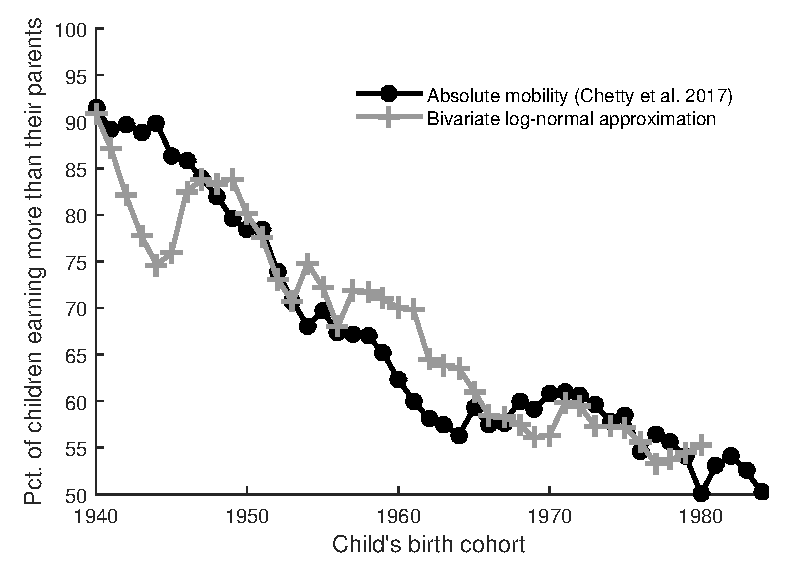
\includegraphics[width=1.0\textwidth] {./figs/trend1.eps}
\caption{A comparison between the measured (black) and approximated absolute mobility (gray). A bivariate normal distribution reproduces the historical trend of the rate of absolute mobility (the calculations are based on the pre-tax income per capita and pre-tax income distribution reported in~\citet{PikettyZucman2014} and~\citet{WID2017} assuming fixed correlation of $\rho=0.57$).}
\flabel{trend}
\end{figure}

The canonical measure of relative intergenerational mobility is the elasticity of child income with respect to parent income, known as the intergenerational earnings elasticity (IGE)~\citep{mulligan1997parental,lee2009trends,chetty2014land}. IGE is a measure of immobility rather than of mobility: the larger it is, the stronger the relationship between parent and child income. Therefore, $1-\beta$ is used as a measure of mobility. Unlike absolute mobility, empirical studies of IGE and other relative mobility measures in the United States show them holding stable over recent decades~\citep{lee2009trends,hauser2010intergenerational,chetty2014land,chetty2014united}.

Co-observations of declining absolute mobility and stable relative mobility are seemingly contradictory and require careful interpretation. The explanation of~\citet{chetty2017fading} for the contrast is that income growth has been unequally distributed -- positive for high earners and stagnant for the rest -- meaning that aggregate income growth has contributed little to absolute mobility. This finding is consistent with their data but may not describe the only mechanism at work. Here we note a theoretical relationship between relative and absolute mobility, which suggests that their co-movement should not, in general, be expected.

\section{Model}

Our starting point is a population of $N$ parent-child pairs. We denote by $Y_p^i$ and $Y_c^i$ the incomes of the parent and the child (at the same age), respectively, in family $i=1\dots N$. We assume the incomes are all positive and define the log-incomes $X_p^i=\log Y_p^i$ and $X_c^i=\log Y_c^i$.

The intergenerational earnings elasticity (IGE) is defined as the slope ($\beta$) of the linear regression

\be
X_c = \alpha + \beta X_p + \epsilon\,,
\ee
where $\alpha$ is the regression intercept and $\epsilon$ is the error term.

The rate of absolute mobility, denoted by $A$, as defined and measured by~\citet{chetty2017fading} is the fraction of children earning more than their parents, equal to the probability $P\left(X_c-X_p > 0\right)$.

One hypothetical sample of the joint parents and children log-income distribution is presented in~\fref{lines}.~\fref{lines} also depicts how $A$ and $\beta$ are defined -- the blue line is $y=x$, hence the rate of absolute mobility is defined as the fraction of parent-child pairs which are above it. The red line is the linear regression $y=\alpha +\beta x$, for which $\beta$ is the IGE.

\begin{figure}[!htb]
\centering
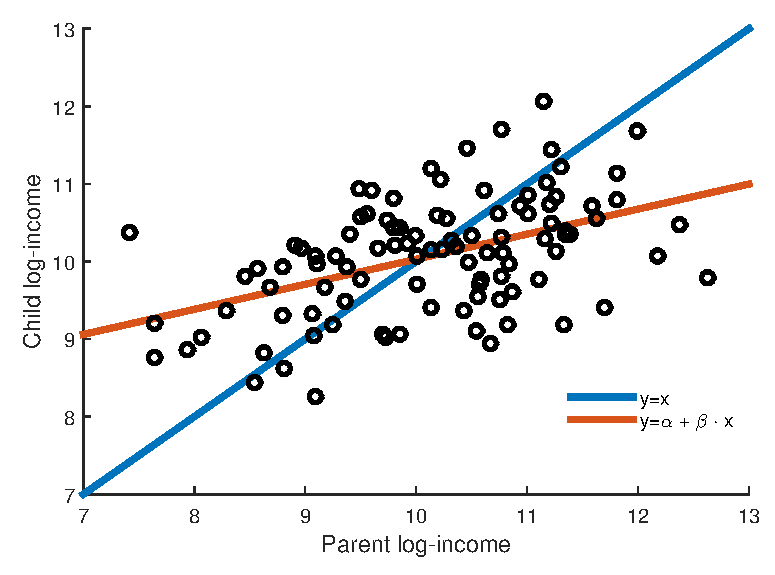
\includegraphics[width=1.0\textwidth]{./figs/bivariate_lines3.eps}
\caption{An illustration of the absolute and relative mobility measures. The black circles are a randomly chosen sample of 100 parent-child log-income pairs, assuming a bivariate normal distribution. The parameters used were $\mu_p=10.1$, $\sigma_p=0.78$ (for the parents marginal distribution) and $\mu_c=10.25$, $\sigma_c=1.15$ (for the children marginal distribution) with correlation of $\rho=0.57$. The resulting $\alpha$ and $\beta$ were $1.8$ and $0.84$, respectively.}
\flabel{lines}
\end{figure}

Since income distributions are known to be well approximated by the log-normal distribution~\citep{pinkovskiy2009parametric}, a simple plausible model for the joint distribution of parent and child log-incomes is the bivariate normal distribution. Under this assumption, the marginal income distributions of both parents and children are log-normal and the correlation between their log-incomes is defined by a single parameter $\rho$. The marginal distributions of the parents and the children follow $\mathcal{N}\left(\mu_p,\sigma_p^2\right)$ and $\mathcal{N}\left(\mu_c,\sigma_c^2\right)$, respectively. Hence the joint distribution is fully characterized by 5 parameters: $\mu_p$, $\sigma_p$, $\mu_c$, $\sigma_c$ and $\rho$.

\section{Results}

We first address the properties of the bivariate normal approximation. In particular, we derive close form expressions for both measures of mobility, $A$ and $1-\beta$, in terms of the distribution parameters:

\begin{proposition}
\label{prop:prop1}

For a bivariate normal distribution with parameters $\mu_p$, $\sigma_p$ (for the parents marginal distribution) and $\mu_c$, $\sigma_c$ (for the children marginal distribution) assuming correlation $\rho$, the IGE is

\be
1-\beta = 1-\frac{\sigma_c}{\sigma_p}\rho \,.
\elabel{beta_rho}
\ee
\end{proposition}

Following \pref{prop1} it is also possible to derive the rate of absolute mobility as a function of the distribution parameters and the IGE:

\begin{proposition}
\label{prop:prop2}

For a bivariate normal distribution with parameters $\mu_p$, $\sigma_p$ (for the parents marginal distribution), $\mu_c$, $\sigma_c$ (for the children marginal distribution) and $\rho=\sigma_p\beta/\sigma_c$ (where $\beta$ is the IGE), the rate of absolute mobility is

\be
A = \Phi\left(\frac{\mu_c - \mu_p}{\sqrt{\sigma_p^2\left(1 - 2\beta\right) + \sigma_c^2}}\right) \,,
\elabel{abs2}
\ee
where $\Phi$ is the cumulative distribution function of the standard normal distribution.
\end{proposition}

Our next step is to test whether the bivariate normal model for the joint distribution of the log-incomes is empirically sound. For that purpose we compare the model prediction for the historical rate of absolute mobility in the United States with the historical rate reported by~\citet{chetty2017fading}. We use data for the per capita pre-tax income in the United States~\citep{PikettyZucman2014} and the income share data~\citep{WID2017} to obtain $\mu_p$, $\sigma_p$, $\mu_c$ and $\sigma_c$ every year. Since in the bivariate normal model, the marginal distributions are log-normal, these parameters can be obtained directly and no fit is required. We then use~\eref{beta_rho} and~\eref{abs2} to calculate the historical value of $A$, while fitting the correlation $\rho$ to a fixed value which minimizes the sum of squared errors from the values reported by~\citet{chetty2017fading}.

The gray curve in~\fref{trend} shows that the model reproduces faithfully the evolution of absolute mobility reported by~\citet{chetty2017fading}, despite its comparative methodological naivety.

Having established its empirical soundness, we can use the model's properties to further study the measures of mobility -- $A$ and $1-\beta$.~\pref{prop2} demonstrates that the rate of absolute mobility can be explicitly described as a function of the relative mobility.~\fref{relat} shows $A$ as a function of $1-\beta$ for different birth cohorts in the United States. It shows that the bivariate normal model -- with positive income growth and inequality changes consistent with data, but absent other effects -- predicts an \textit{inverse} relationship between absolute and relative mobility.

\begin{figure}[!htb]
\centering
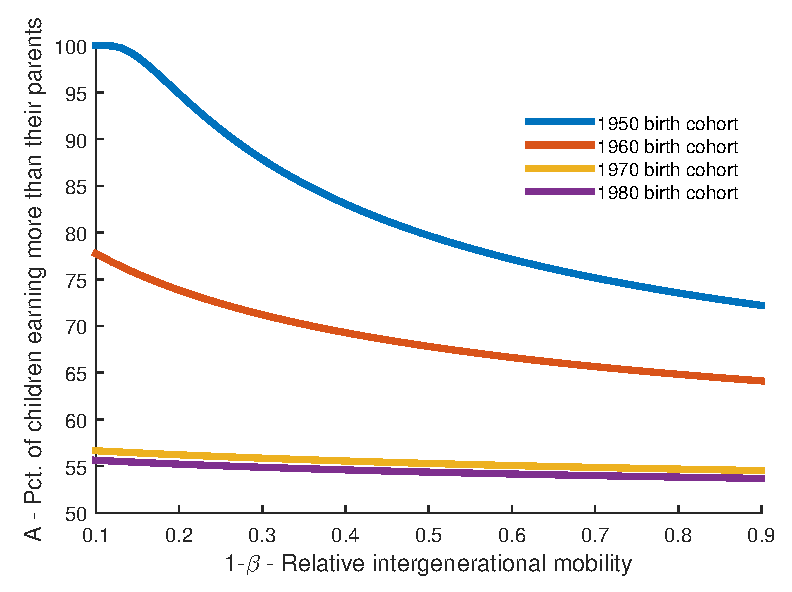
\includegraphics[width=1.0\textwidth] {./figs/relat1.eps}
\caption{The theoretical relationship between the rate of absolute mobility and the complement of the intergenerational earnings elasticity, assuming the bivariate normal log-incomes model for different birth cohorts in the United States. This demonstrates the counterintuitive result that the two mobility measures are inversely related.}
\flabel{relat}
\end{figure}

\Pref{prop2} illustrates that the rate of absolute mobility increases with increasing income growth and decreases with increasing income inequality, as described by~\citet{chetty2017fading}. However, it also demonstrates that an additional mechanism can be at play, since the rate of absolute mobility decreases with increasing relative mobility.

\section{Discussion}

The counterintuitive inverse theoretical relationship found between absolute and relative mobility stems from a fundamental conceptual difference between the two categories of mobility. It exposes the problems that can arise if both are treated as measuring similarly the same phenomenon. In particular, absolute mobility is very sensitive to across-the-board economic growth. For example, during the Middle Ages -- when relative mobility rates were low because social class and profession were predominantly inherited~\citep{goldthorpe1982social,clark2014also}, even the slightest positive or negative income growth would result in very high or low absolute mobility. A misleading picture of intergenerational mobility may arise if the basic properties of these measures are overlooked. Therefore, empirically addressing concepts like the ``American Dream''~\citep{corak2009chasing,chetty2017fading} and equality of opportunity~\citep{roemer2000opportunity,chetty2014land} requires careful delineation of the phenomena of interest and the manner in which quoted measures reflect them.

\clearpage

\doublespacing
\bibliography{mobmob}

\clearpage

\doublespacing

\appendix

\section{Proofs}

\subsection{Proof of \preflong{prop1}}

First, by definition, the correlation $\rho$, between $X_p$ and $X_c$ equals to their covariance, divided by $\sigma_p\sigma_c$

\be
\rho = \frac{\text{Cov}\left[X_p,X_c\right]}{\sigma_p\sigma_c}\,.
\ee

$\beta$ can be directly calculated as follows, by the linear regression slope definition:

\be
\beta = \frac{\sum_{i=1}^{N} {\left(X_p^i - \bar{X}_p\right)\left(X_c^i - \bar{X}_c\right)}}{\sum_{i=1}^{N} {\left(X_p^i - \bar{X}_p\right)}}\,,
\ee
where $\bar{X}_p$ and $\bar{X}_c$ are the average parents and children log-incomes, respectively.

It follows that 
\be
\beta = \frac{\text{Cov}\left[X_p,X_c\right]}{\sigma_p^2}\,.
\ee

We immediately obtain

\be
\beta = \frac{\sigma_c}{\sigma_p}\rho
\ee

and therefore

\be
1-\beta = 1-\frac{\sigma_c}{\sigma_p}\rho
\ee

\qed

\subsection{Proof of \preflong{prop2}}

We start by defining a new random variable $Z = X_c-X_p$. It follows that calculating $A$ is equivalent to calculating the probability $P\left(Z>0\right)$.

Subtracting two dependent normal distributions yields that

\be
Z \sim \mathcal{N}\left(\mu_c - \mu_p,\sigma_p^2 + \sigma_c^2 - 2\text{Cov}\left[X_p,X_c\right]\right)\,,
\ee

so according to \pref{prop1}

\be
Z \sim \mathcal{N}\left(\mu_c - \mu_p,\sigma_p^2\left(1-2\beta\right) + \sigma_c^2\right)\,.
\ee

If follows that

\be
\frac{Z - \left(\mu_c - \mu_p\right)}{\sqrt{\sigma_p^2\left(1-2\beta\right) + \sigma_c^2}} \sim \mathcal{N}\left(0,1\right)\,,
\ee

so we can now write

\be
\begin{split}
&P\left(Z>0\right) = \\ & P\left(\frac{Z - (\mu_c - \mu_p)}{\sqrt{\sigma_p^2\left(1-2\beta\right) + \sigma_c^2}} > -\frac{\mu_c - \mu_p}{\sqrt{\sigma_p^2\left(1-2\beta\right) + \sigma_c^2}} \right) = \\ &\Phi\left(\frac{\mu_c - \mu_p}{\sqrt{\sigma_p^2\left(1 - 2\beta\right) + \sigma_c^2}}\right) \,,
\end{split}
\ee
where $\Phi$ is the cumulative distribution function of the standard normal distribution.

\qed

\end{document}